\large
The feedforward system uses a Filtered-$x$ Least Mean Square (FXLMS) algorithm:
\begin{equation}
b_j[n+1] = b_j[n] - 2\mu e[n] \cdot f[n-j]
\end{equation}



The algorithm adapts the impulse response of the control filter, outputting a counterphase signal. \cite{HansenSnyder}

\vspace{2mm}

\resizebox{1\columnwidth}{!}{
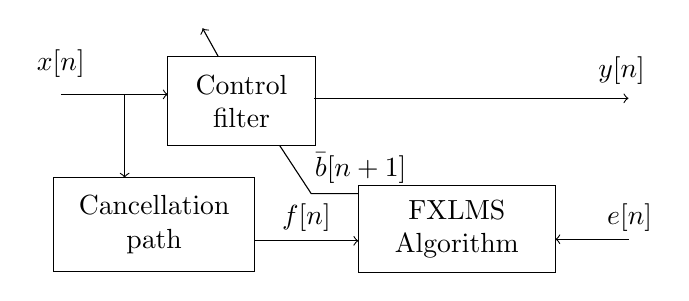
\begin{tikzpicture}
\draw  (-2.9,0.98) rectangle node[text width=2.5cm,align=center] {\textrm{Cancellation \\ path}}(-0.35,-0.21);
\draw  (0.97,0.88) rectangle node[text width=2.5cm,align=center] {\textrm{FXLMS Algorithm}} (3.47,-0.22);
\draw  (-1.45,2.52) rectangle node[text width=1.5cm,align=center,fill=white] {\textrm{Control filter}} (0.42,1.39);
\draw[->] (-0.35,0.18) -- node[above]{$f[n]$} (0.97,0.18);
\draw [->](-2,2.03) -- (-2,0.98);
\draw [->](-2.81,2.04) node[left,above=2.5]{$x[n]$} -- (-1.45,2.04);
\draw[->] (0.41,1.99) -- (1.25,1.99) -- (4.4,1.99) node[left=2.5,above=1.5]{$y[n]$};
\draw (0.97,0.78) -- (0.37,0.78) --node[above=0.55,right=3.5]{$\bar{b}[n+1]$} (-0.03,1.39);
\draw [->](-0.81,2.52) -- (-1.01,2.88);
\draw[->] (4.4,0.2) -- node[above=8,right=2]{$e[n]$} (3.47,0.2);
\end{tikzpicture}
}

\vspace{2mm}

Wiener filtering is used for LP of future samples, using the Wiener-Hopf equation:
\begin{equation}
\hat{R}\bar{a} = -\bar{\hat{r}}_x
\end{equation}



Where the characteristics of speech are determined in a frame based autocorrelation function (ACF). \cite{SpeechCoding}

%\vspace{-2mm}
%\begin{equation*}
%	PG = 10 log_{10}\bigg(\frac{\sigma^2_x}{\sigma^2_\varepsilon}\bigg)
%%\end{equation*}

\vspace{1mm}

\resizebox{1\columnwidth}{!}{
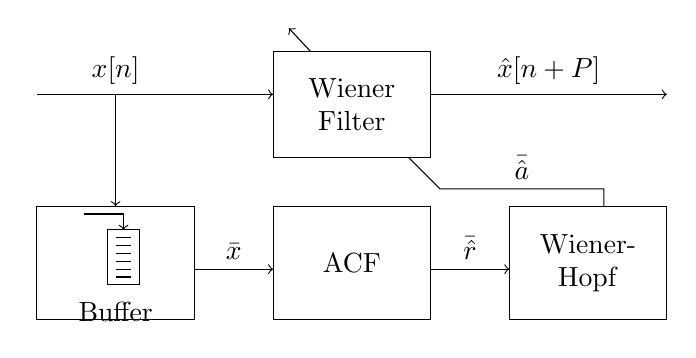
\begin{tikzpicture}

%% Boxes
\draw  (-3,3) rectangle node[text width=2cm,align=center] {\textrm{Wiener Filter}}(-1,4.34);
\draw  (-1,2.38) rectangle node[text width=2cm,align=center] {\textrm{ACF}}(-3,0.94);
\draw  (-4,2.38) rectangle node[text width=2cm,align=center,below=10.55] {\textrm{Buffer}}(-6,0.94);
\draw  (0,2.38) rectangle node[text width=1.5cm,align=center] {\textrm{Wiener- Hopf}}(2,0.94);



%%Buffer
\draw (-4.7,1.38) node (v1) {} -- (-5.1,1.38) -- (-5.1,2.08) -- (-4.7,2.08) -- (-4.7,1.38);
\draw (-5,1.98) -- (-4.8,1.98);
\draw (-5,1.88) -- (-4.8,1.88);
\draw (-5,1.78) -- (-4.8,1.78);
\draw (-5,1.68) -- (-4.8,1.68);
\draw (-5,1.58) -- (-4.8,1.58);
\draw (-5,1.48) -- (-4.8,1.48);
\draw [->](-5.4,2.28) -- (-4.9,2.28) -- (-4.9,2.08);


%% Lines
\draw [->](-4,1.58) -- node[above]{$\bar{x}$} (-3,1.58);
\draw [->](-1,1.58) -- node[above]{$\bar{\hat{r}}$}(0,1.58);
\draw (1.2,2.38) -- (1.2,2.6) -- node[above]{$\bar{\hat{a}}$} (-0.88,2.6) -- (-1.28,3);


\draw [->](-2.52,4.34) -- (-2.8,4.64);
\draw [->](-6,3.8) node[right,above]{} -- (-3,3.8);
\draw [->](-5,3.8) node[above]{$x[n]$} -- (-5,2.38);
\draw [->](-1,3.8) --  node[above]{$\hat{x}[n+P]$}(2,3.8);
\end{tikzpicture}}





